% article.tex, a sample LaTeX file.
% Run LaTeX on this file twice for proper section numbers.
% A '%' causes LaTeX to ignore remaining text on the line

% Use the following line for draft mode (double spaced, single column)
\documentclass[preprint,pre,floats,aps,amsmath,amssymb]{revtex4}



% Use the following line for journal mode (single spaced, doublecolumn)
%\documentclass[twocolumn,pre,floats,aps,amsmath,amssymb]{revtex4}
\usepackage{graphicx}

\usepackage{bm}
\usepackage{enumerate}
\usepackage{wrapfig}
\usepackage{amsmath}
\usepackage{float}
\begin{document}


\title{scientific report: Quick Sort implementation on MS\_MPI 
}
\author{Ammar Ali Master Student}
\affiliation{Department Of Information Technology And Programming,Business Information System,ITMO University, Saint Petersburg  RUSSIA}
\date{\today}



\newpage
\begin{abstract}
	
In this report, we will present a quick sort algorithm. We will go through the quick sort algorithm which holds for $O(N.log(N))$ time complexity in average case and $O(N^2)$ in the worst case. Then we will discuss the Microsoft Messaging Passing Interface (MPI) library which we will use to implement the quick sort algorithm based on multi-threading instead of running on one thread and it will be implemented to our recursion function of quicksort. Then we will discuss how the multi-threading will affect the run-time.
  
\end{abstract}

\maketitle

\section{Introduction}
\label{sec:intro}
Quicksort is similar to merge sort as both are divide and conquer algorithms. Quicksort idea is picking an element as a pivot and make a partition of the array around the picked pivot.
And this process will go recursively partition reordering the elements according to the picot and so one.
Noticing that, at each level, we are generating two partitions that are not sequential which means we can assign a full branch to a thread and the other one to a thread. Going from this idea we will implement our multi-threading program using MS-MPI.    

\section{Discussion}
	\label{sec:Discussion}
\subsection{Quick Sort Using One Thread}
As we mentioned that the quicksort is a divide and conquer problem and the main idea is to make partitions according to pivot elements. It is nice to mention how we propose an element as a pivot. Actually, there are multiple versions to quick sort which differs in the way of choosing the pivot elements. Always pick the first or the last element as pivot or maybe randomly as well the median could be used to make sure that the partitions are equal and we have a balanced tree but that doesn't mean it is better because it always depends on the distribution of the elements and always the worst case will have $O(n^2)$ complexity.And I am picking the last element as a pivot on my implementation. 
the main process in quicksort that in linear time we should choose our pivot and reorder the array in a way that all the left-handed elements of the pivot are smaller and all the right side elements are bigger.
we can represent the complexity of the quick sort algorithm like the following:
$$ F(n) = F(k) + F(n-k-1)+\psi(n) $$
where $F(n)$ is the time taken to sort an array of length n and k is the number of elements smaller than the pivot and $\psi(n)$  is related to the partition process.so if we choose the pivot as a median for example that will give as better performance for $F(k)$ but could affect $\psi(n)$ in a bad way because if the median was always the biggest or smallest element the worst case will occur.in my implementation the worst case will be if the array was already sorted in increasing or decreasing order then:
$$ F(n) = F(0) + F(n-1) +\psi(n)\;\; \implies \;\; F(n)=F(n-1)+\psi(n)$$
the above equation holds a solution of the above recurrence $\psi(n^2)$.
 
\subsection{MS-MPI and Quick Sort Using Multi-Threading}
Thanks to parallel computing which allowed us to compute Sorting in less time needed.
I used MS-MPI (Microsoft Message Passing Interface) to parallelize quick sort on my implementation to share the sorting data among multiple processes.
\begin{figure}[h]
	\centering
	\caption{Basic Steps} 
	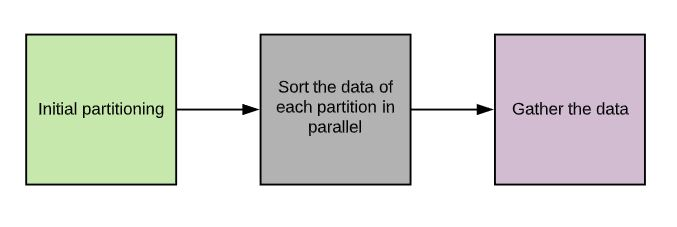
\includegraphics[scale=0.5]{1}
\end{figure}
In fig(1), We simplify our basic idea used in the implementation. Going through an initial partition as long as we still have available processes then each processor or thread will have an array and will apply the sequential quick sort on these arrays in parallel each thread with its array. And all these arrays are partitions from the main input array. Then we will gather all the data by sending locally sorted data to its original sender.we will use the rank (thread id) to allocate data considering.
Thread T with id R will share its partition with the process rank equals to the process id adding two to the power of the recursion depth so the processes are allocated using this formula \cite{quicksort}.
The sharing partition is chosen to be the one that includes the smaller set because that will reduce the number of communications. Also, the process that computes partition will be the next in line to share the data again before the receiving process. If any more processes are in the pool the sending process has more chances in sharing its data than the receiving process.

\newpage      
\section{Implementation}
\label{sec:implementation }
The code will be attached to the report.


\section{Results}
\label{sec:results}
\begin{figure}[h]
	\centering
	\caption{run-time according to number of used threads}
	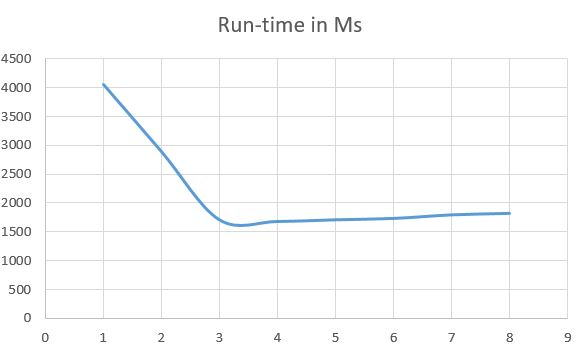
\includegraphics[scale=0.5]{2} 
	
\end{figure}
I generated $100000$ random numbers between 1 and 100 and run the code on a different number of threads as shown in fig(2). The best Running Time obtained when the number of threads equals 4 and for more threads, the run-time started to increase again.
Note:
tor run the code please using command window go to the directory of the debug in the project folder and type:\newline
mipexec -n 4 MPIfirst\newline
or specify any number of threads you want. Also maybe a conflict occurs because of using $ freopen$ to read from files.To solve this problem please add " \_CRT\_SECURE\_NO\_WARNINGS" to the $ Project\; Properties\; ->\; C/C++\;->\;Preprocessor\;->\;Preprocessor\;Definitions $. 

\newpage


\begin{thebibliography}{9}
	\section{Reference}
	\bibitem{quicksort} 
 
	[\textit{https://www.codeproject.com/Articles/42311/Parallel-Quicksort-using-MPI-Performance-Analysis }]. 

	

	
\end{thebibliography}
\appendix*



\end{document}             % End of document.

